%% abtex2-modelo-trabalho-academico.tex, v-1.9.2 laurocesar
%% Copyright 2012-2014 by abnTeX2 group at http://abntex2.googlecode.com/ 
%%
%% This work may be distributed and/or modified under the
%% conditions of the LaTeX Project Public License, either version 1.3
%% of this license or (at your option) any later version.
%% The latest version of this license is in
%%   http://www.latex-project.org/lppl.txt
%% and version 1.3 or later is part of all distributions of LaTeX
%% version 2005/12/01 or later.
%%
%% This work has the LPPL maintenance status `maintained'.
%% 
%% The Current Maintainer of this work is the abnTeX2 team, led
%% by Lauro César Araujo. Further information are available on 
%% http://abntex2.googleco@misc{MarileneCarneiroMatos,

%%
%% This work consists of the files abntex2-modelo-trabalho-academico.tex,
%% abntex2-modelo-include-comandos and abntex2-modelo-references.bib
%%
% ------------------------------------------------------------------------
% ------------------------------------------------------------------------
% abnTeX2: Modelo de Trabalho Academico (tese de doutorado, dissertacao de
% mestrado e trabalhos monograficos em geral) em conformidade com 
% ABNT NBR 14724:2011: Informacao e documentacao - Trabalhos academicos -
% Apresentacao
% ------------------------------------------------------------------------
% ------------------------------------------------------------------------


%Testando o git

\documentclass[
% -- opções da classe memoir --
    12pt,                % tamanho da fonte
    openright,            % capítulos começam em pág ímpar (insere página vazia caso preciso)
    oneside,            % para impressão em verso e anverso. Oposto a oneside
    a4paper,            % tamanho do papel.
% -- opções da classe abntex2 --
%chapter=TITLE,		% títulos de capítulos convertidos em letras maiúsculas
%section=TITLE,		% títulos de seções convertidos em letras maiúsculas
%subsection=TITLE,	% títulos de subseções convertidos em letras maiúsculas
%subsubsection=TITLE,% títulos de subsubseções convertidos em letras maiúsculas
% -- opções do pacote babel --
    english,            % idioma adicional para hifenização
    brazil,                % o último idioma é o principal do documento
]{abntex2}

% ---
% Pacotes básicos 
% ---
\usepackage{unitins}
\usepackage{lmodern}            % Usa a fonte Latin Modern
\usepackage[T1]{fontenc}        % Selecao de codigos de fonte.
\usepackage[utf8]{inputenc}        % Codificacao do documento (conversão automática dos acentos)
\usepackage{lastpage}            % Usado pela Ficha catalográfica
\usepackage{indentfirst}        % Indenta o primeiro parágrafo de cada seção.
\usepackage{color}                % Controle das cores

\usepackage{graphicx}
\usepackage{float}
\usepackage[export]{adjustbox}  % Inclusão de gráficos
\usepackage{subfig}
\usepackage{microtype}            % para melhorias de justificação
\usepackage{soul}
\usepackage{amssymb}
\usepackage{amsmath}
\usepackage{spreadtab}
\usepackage{multirow}
\usepackage{amsthm}
\usepackage{url}
\usepackage[portuguese, ruled, linesnumbered]{algorithm2e}

\usepackage{listings}           % Pacote para utilização de código fonte


% ---

% ---
% Pacotes adicionais, usados apenas no âmbito do Modelo Canônico do abnteX2
% ---
\usepackage{lipsum}                % para geração de dummy text
% ---

% ---
% Pacotes de citações
% ---

% \usepackage[brazilian,hyperpageref]{backref}	 % Paginas com as citações na bibl
\usepackage[alf,abnt-etal-list=2 ]{abntex2cite}    % Citações padrão ABNT


\usepackage[table]{xcolor}
\definecolor{lightgray}{gray}{0.9}
\graphicspath{{Imagens/}}

\theoremstyle{theorem}
\newtheorem{teo}{Teorema}[chapter]
\newtheorem{lema}[teo]{Lema}
\theoremstyle{definition}
\newtheorem{defi}[teo]{Definição}


% --- 
% CONFIGURAÇÕES DE PACOTES
% --- 

% ---
% Configurações do pacote backref
% Usado sem a opção hyperpageref de backref
% \renewcommand{\backrefpagesname}{Citado na(s) página(s):~}
% Texto padrão antes do número das páginas
% \renewcommand{\backref}{}
% Define os textos da citação
% \renewcommand*{\backrefalt}[4]{
% 	\ifcase #1 %
% 		Nenhuma citação no texto.%
% 	\or
% 		Citado na página #2.%
% 	\else
% 		Citado #1 vezes nas páginas #2.%
% 	\fi}%
% ---

% ---
% Informações de dados para CAPA e FOLHA DE ROSTO
% ---
\titulo{Reconhecimento Facial}
\autor{Luan Coêlho de Souza}
\local{Palmas}
\data{2023}
\orientador{Prof. Jânio Elias Teixeira Júnior}
\instituicao{%
    Universidade Estadual do Tocantins

    Curso de Sistemas de Informação
}
\tipotrabalho{Estágio Supervisionado (Graduação)}
% O preambulo deve conter o tipo do trabalho, o objetivo, 
% o nome da instituição e a área de concentração 
\preambulo{Projeto apresentado como requisito para aprovação
na disciplina de Estágio Supervisionado do Curso de
Sistemas de Informações da Universidade Estadual
do Tocantins - UNITINS, sob a Orientação do Prof. Me. Jânio Elias Teixeira Junior.}

% ---


% ---
% Configurações de aparência do PDF final

% alterando o aspecto da cor azul
\definecolor{blue}{RGB}{41,5,195}

% informações do PDF

\hypersetup{
%pagebackref=true,
    pdftitle={\@title},
    pdfauthor={\@author},
    pdfsubject={\imprimirpreambulo},
    pdfcreator={LaTeX with abnTeX2},
    pdfkeywords={Algoritmo}{trabalho acadêmico},
    colorlinks=true,            % false: boxed links; true: colored links
    linkcolor=blue,            % color of internal links
    citecolor=blue,                % color of links to bibliography
    filecolor=magenta,            % color of file links
    urlcolor=blue,
    bookmarksdepth=4
}

% --- 

% --- 
% Espaçamentos entre linhas e parágrafos 
% --- 

% O tamanho do parágrafo é dado por:
\setlength{\parindent}{1.3cm}

% Controle do espaçamento entre um parágrafo e outro:
\setlength{\parskip}{0.2cm}  % tente também \onelineskip

% ---
% compila o indice
% ---
\makeindex
% ---

% ----
% Início do documento
% ----
\usepackage{pdfpages}
\begin{document}

% Retira espaço extra obsoleto entre as frases.
    \frenchspacing

% ----------------------------------------------------------
% ELEMENTOS PRÉ-TEXTUAIS
% ----------------------------------------------------------
%  \pretextual
% ----------------------------------------------------------

%  \pagestyle{headings}
    \pagestyle{simple}


    % ----------------------------------------------------------
% ELEMENTOS PRÉ-TEXTUAIS
% ----------------------------------------------------------

% \pretextual

% ---
% Capa
% ---
\imprimircapa
% ---

% ---
% Folha de rosto
% (o * indica que haverá a ficha bibliográfica)
% ---
\imprimirfolhaderosto
% ---

% ---
% Inserir folha de aprovação
% ---

% Isto é um exemplo de Folha de aprovação, elemento obrigatório da NBR
% 14724/2011 (seção 4.2.1.3). Você pode utilizar este modelo até a aprovação
% do trabalho. Após isso, substitua todo o conteúdo deste arquivo por uma
% imagem da página assinada pela banca com o comando abaixo:
%
% \includepdf{folhadeaprovacao_final.pdf}
%
\begin{folhadeaprovacao}

  	
  	
  	\begin{center}
  		
\includegraphics[width=1\textwidth]{imagens/unitins}
  		\ABNTEXchapterfont\Large   CURSO DE SISTEMAS DE INFORMA{Ç}{Ã}O
  		

  		\vspace*{1cm}     
  		{\ABNTEXchapterfont\bfseries\large \expandafter\MakeUppercase{\imprimirtitulo}  \vspace*{1cm}    }

  		{\large \expandafter\MakeUppercase{\imprimirautor}}
  		%\vspace*{\fill}

  		\vspace*{1cm}     
  		\hspace{.45\textwidth}
  		\begin{minipage}{.5\textwidth}
  			\small\imprimirpreambulo
  			
  		\end{minipage}%
  	%	\vspace*{\fill}
  	\end{center}
  
        
  \assinatura{\textbf{Estagiário (a)}}
  \assinatura{\textbf{Supervisor (a) da Concedente ou Responsável pela Supervisão no Laboratório}}
   \assinatura{\textbf{\imprimirorientador} \\ Orientador} 
   
   
      
   \begin{center}
    \vspace*{0.5cm}
    {\large\imprimirlocal}

    {\large\imprimirdata}
    \vspace*{1cm}
  \end{center}
  
\end{folhadeaprovacao}


% ---
% RESUMOS
% ---

% resumo em português
\setlength{\absparsep}{18pt} % ajusta o espaçamento dos parágrafos do resumo
\begin{resumo}



 \textbf{Palavras-chaves}: 
 
\end{resumo}

% resumo em inglês
\begin{resumo}[Abstract]
 \begin{otherlanguage*}{english}
 
   \vspace{\onelineskip}
 
   \noindent 
   \textbf{Key-words}:
 \end{otherlanguage*}
\end{resumo}


% ---
% inserir lista de ilustrações
% ---
\pdfbookmark[0]{\listfigurename}{lof}
\listoffigures*

% ---


% ---
% inserir lista de abreviaturas e siglas
% ---
\begin{siglas}
\item API - \textit{Application Programming Interface}
\item HTTP - \textit{Hypertext Transfer Protocol}
\item JSON - \textit{JavaScript Object Notation}
\item OEM - \textit{Original Equipment Manufacturer}
\item REST - \textit{Representational State Transfer Protocol}
\item SDK - \textit{Software Development Kit}
\item  SOAP - \textit{Simple Object Access Protocol}
\item SO - Sistema Operacional
\item WSDL - \textit{Web Services Description Language}
\item XML - \textit{Extensible Markup Language}
  
  
  
\end{siglas}
% ---


% ---
% inserir o sumario
% ---
\pdfbookmark[0]{\contentsname}{toc}
\tableofcontents*
\cleardoublepage
% ---



% ELEMENTOS TEXTUAIS
% ---------------------------------[!htb]-------------------------

    \textual

%Capitulos
    % ----------------------------------------------------------
% Introdução (exemplo de capítulo sem numeração, mas presente no Sumário)
% ----------------------------------------------------------

\chapter{Introdução}\label{ch:intro}


\section{Objetivos}\label{sec:objetivos}

\subsection{Objetivo Geral}\label{subsec:objetivo-geral}

\subsection{Objetivos Específicos}\label{subsec:objetivos-especificos}
\begin{itemize}

    \item
    \item
    \item

\end{itemize}

    % ---
% Capitulo de revisão de literatura
% ---


\chapter{Referencial Teórico}\label{ch:referencial_teorico}


\section{Autenticação e Identidade}\label{sec:autenticacaoeidentidade}
O problema de estabelecer uma associação entre um indivíduo e uma identidade pode ser dividido em duas categorias: autenticação e identificação~\cite{magalhaes2003biometria}.

\subsection{Autenticação}\label{subsec:autenticacao}
É o processo que verifica a autenticidade de um usuário, processo ou dispositivo.
Essa verificação confirma a legitimidade da entidade em questão.
Durante a autenticação, a parte que examina assegura que a entidade sendo verificada é genuína, e esta última participa ativamente na troca de informações~\cite{usmonov2021identification}.


Para~\cite{conti2017biometric} existem três tipos de autenticação\label{tipos-autenticacao}:

\begin{itemize}
    \item \textbf{Baseada em conhecimento:} utiliza informações que a pessoa sabe, como uma senha.
    \item \textbf{Com base em algo que a pessoa possua}, como um \textit{token} ou cartão inteligente.
    \item \textbf{Com base em características físicas da pessoa}, também conhecidas como biometria.
\end{itemize}


\section{Biometria}\label{sec:biometria}
O termo \("\)biometria\("\) vem das palavras gregas \("\)bios\("\) (vida) e \("\)metrikos\("\) (medida)~\cite{magalhaes2003biometria}.
É o estudo que visa identificar um indivíduo com base em suas características fisiológicas e comportamentais~\cite{handa2019comparative}, ou seja, biometria é uma forma de identificar pessoas usando características físicas ou comportamentais únicas.

Dos tipos mencionados em~\ref{tipos-autenticacao}, a biometria é tida como a abordagem mais segura, já que os atributos físicos de uma pessoa não podem ser furtados, cedidos ou esquecidos.
Falsear a autenticação biométrica é complicado e inviável, uma vez que avalia características singulares do indivíduo~\cite{dos2019tecnologias}.

\subsection{Tecnologias Biométricas}\label{subsec:biometria-tecnologias}

\subsubsection{Reconhecimento facial}\label{subsubsec:reconhecimento-facial}
É uma tecnologia capaz de identificar uma pessoa a partir de uma imagem digital ou de um vídeo, de modo que é comparado as características faciais selecionadas de uma determinada imagem com os rostos existentes numa base de dados~\cite{orvalho2019reconhecimento}.
Essas características incluem a distância entre os olhos, largura do nariz, posição das maçãs do rosto, linha da mandíbula, queixo, entre outras~\cite{adeoye2010survey}.
%O rosto não possui tantos traços únicos mensuráveis quanto impressões digitais ou íris dos olhos, o que faz com que a confiabilidade do reconhecimento facial seja levemente inferior a desses outros métodos biométricos.
%
%No entanto, ainda é adequado para muitas aplicações, especialmente pela sua conveniência para o usuário.
%O reconhecimento facial também pode ser utilizado em conjunto com o reconhecimento de impressões digitais ou outro método biométrico para desenvolver aplicações com necessidades de segurança mais críticas

%\begin{longtable}[c]{|l|l|}
    \hline
    \multicolumn{1}{|c|}{\textbf{Problemas}} & \multicolumn{1}{c|}{\textbf{Reconhecimento Facial}} \\ \hline
    \endfirsthead
    \endhead
    Sensor & \begin{tabular}[c]{@{}l@{}}
                 Resolução espacial, taxa\\ de quadros, distância da\\ câmera.
    \end{tabular} \\ \hline
    Envelhecimento & \begin{tabular}[c]{@{}l@{}}
                         Mudanças geométricas\\ entre a infância e a\\ adolescência, rugas e\\ flacidez facial.
    \end{tabular} \\ \hline
    Interação com o usuário & Poses e expressões. \\ \hline
    \begin{tabular}[c]{@{}l@{}}
        Mudanças no meio\\ ambiente
    \end{tabular} & \begin{tabular}[c]{@{}l@{}}
                        iluminação e cena de\\ fundo.
    \end{tabular} \\ \hline
    Outros fatores & \begin{tabular}[c]{@{}l@{}}
                         Maquiagem, acessórios,\\ e oclusão
    \end{tabular} \\ \hline
    \caption*{Fonte: Adaptado de~\cite{usmonov2021identification}}
\end{longtable}


\subsubsection{Reconhecimento da Geometria da Mão}\label{subsubsec:geometria-mao}
O reconhecimento da geometria da mão se dá pela análise de características específicas como forma, comprimento dos dedos e linhas distintas.
A segurança deste sistema pode variar dependendo do uso dessas características isoladamente, da sua posição em relação a um ponto fixo ou pela associação de vários pontos e respectivas distâncias a esses características~\cite{magalhaes2003biometria}.

É importante notar que, conforme os estudos~\cite{magalhaes2003biometria}, não há evidências de que a geometria da mão, conforme interpretada pelos algoritmos atuais, seja exclusiva a cada pessoa.
Além disso, em comparação com outras medidas biométricas, a geometria da mão gera um volume menor de dados.
Isso significa que, em uma base de dados ampla, pode ser difícil distinguir indivíduos com características manuais muito similares usando somente a geometria da mão.

\section{Localização Exterior - GPS}\label{sec:localizacao}
GPS é a sigla da abreviatura de \textit{Global Positioning System}, ou Sistema de Posicionamento Global em português~\cite{gpsdesigning}.
Também chamado de NAVSTAR-GPS (Sistema de Navegação por Satélites com Tempo e Distância), é um sistema de navegação por rádio criado pelo Departamento de Defesa dos EUA. Foi criado originalmente para a navegação militar americana~\cite{novais2014localizaccao}.

É o método de identificar a posição geográfica de um objeto, pessoa ou dispositivo eletrônico.
Para isso, utiliza-se de informações provenientes de sinais de~\hypertarget{receptores}{GPS, torres de celular, endereços \textit{IP} ou redes  \textit{Wi-Fi}}.
Em resumo, permite o rastreamento em tempo real da localização de uma entidade~\cite{da2019sistemas}.

O GPS consiste em uma constelação de 24 satélites que orbitam a Terra a uma altitude aproximada de 20.200 km acima do nível do mar.
Essa configuração permite que os~\hyperlink{receptores}{receptores} determinem sua posição em qualquer lugar do planeta com notável precisão~\cite{el2002introduction}.

\subsection{Localização Interna - (Indoor)}\label{subsec:localizacao-indoor}

É uma tecnologia projetada para localização em ambientes internos, como andares de prédios, tuneis, salas ou auditórios~\cite{mittelstadt2018bluepath}.
Um dos fatores que aumentam a confiabilidade da localização de uma pessoa ou objeto em um determinado local é o GPS, entretanto essa tecnologia apresenta melhor desempenho em ambientes abertos, tendo uma grande imprecisão em ambientes fechados.

Quando um receptor está em um espaço interno, torna-se muito difícil decodificar os sinais GPS, uma vez que eles são atenuados por edifícios e paredes.
Isso resulta em perda de potência do sinal e, consequentemente, em erros na localização do receptor.
Nesse contexto, existe a localização indoor~\cite{mittelstadt2018bluepath}.

\subsubsection{Tecnologias de Localização Indoor}\label{subsubsec:tecnologias-localizacao-indoor}
Conforme o entedimento de~\cite{novais2014localizaccao} em sua tese de mestrado \("\)Localização Indoor em Ambientes Inteligentes\("\), ele que explica que as tecnologias de localização indoor geralmente são sem fio, visando uma maior aceitação dos usuários, pois andar com cabos para se localizar em um ambiente não é conveniente.
Dessa forma, as tecnologias wireless proporcionam mais conforto, comodidade e segurança.
Há várias maneiras de prover a localização em ambientes internos, algumas serão explicadas a seguir conforme o autor.

\subsubsubsection{Wi-Fi}\label{subsubsubsec:wifi}
A Wi-Fi (Wireless Fidelity) foi estabelecida em 1999 pela Interbrand\footnote{\url{https://interbrand.com/}} para a Wi-Fi Alliance\footnote{\url{https://www.wi-fi.org/}}, que visa assegurar a compatibilidade entre dispositivos Wi-Fi. Utiliza a norma IEEE 802.11, com acréscimos como os padrões 802.11b/g/n/ac, e permite comunicação entre dispositivos através de ondas de rádio acima de 2.4 GHz. Os pontos de acesso conectam vários dispositivos sem fio e podem comunicar entre si, com alcance de aproximadamente 35 metros em ambientes internos e 110 metros em externos.

A prevalência de redes Wi-Fi em locais públicos e privados facilitou sua adoção em sistemas de localização indoor.
Esses sistemas são específicos para cada edifício e podem guiar pessoas ou robôs com dispositivos móveis Wi-Fi. A precisão aumenta ao limitar as possíveis posições dos dispositivos e fornecer plantas dos locais para reduzir distorções de sinal.

Os sistemas de localização podem operar nos próprios dispositivos (localização implícita) ou em servidores (localização explícita).
A configuração envolve uma fase de treino, coletando intensidade do sinal Wi-Fi e identificadores SSID, e uma fase online que compara os dados recebidos com os mapas de rádio para determinar a posição do dispositivo via técnicas de localização determinísticas ou probabilísticas.

\subsubsubsection{ZigBee}\label{subsubsubsec:zigbee}
ZigBee é um conjunto de protocolos de comunicação de baixa taxa de dados para conexão sem fio de curto alcance, baseado no padrão \textit{IEEE 802.15.4} (É um padrão para redes sem fio de baixo consumo de energia e baixa velocidade de dados, usado em \textit{IoT}) e desenvolvido pela Connectivity Standards Alliance (CSA) \footnote{\url{https://csa-iot.org/}} (anteriormente conhecida como ZigBee Alliance), uma organização sem fins lucrativos.

A tecnologia é econômica e de baixo consumo energético, ideal para automação residencial e monitoramento, mas também é aplicável em localização indoor.
Funciona com rádio frequência e requer a posição conhecida de emissores no ambiente para localizar objetos ou dispositivos através da comunicação entre os emissores.

\subsubsubsection{RFID}\label{subsubsubsec:rfid}
A tecnologia RFID (Radio-Frequency Identification) é usada para armazenar e recuperar dados por meio de transmissão eletromagnética.
O RFID permite identificar e rastrear itens e foi precursor dos sistemas modernos ao identificar aviões amigos ou inimigos.
Um sistema RFID inclui leitores e etiquetas, que comunicam usando frequência de rádio.
Etiquetas passivas não têm bateria e refletem o sinal do leitor com informações moduladas, enquanto etiquetas ativas têm alcance maior, até 100 metros, e são mais rápidas, sendo lidas em menos de 100 milissegundos.

Para localização indoor, RFID é mais complexo, geralmente utilizando o dispositivo móvel como leitor e etiquetas distribuídas como pontos de referência para estimar a localização através do sinal de força recebido (RSSI), exigindo que o edifício seja dividido em zonas para essa finalidade.
    \chapter{Metodologia}\label{ch:metodologia}


\section{Palavras-chave}\label{sec:palavras-chave}
Nesta seção, descrevemos as palavras-chave utilizados na busca bibliográfica para este trabalho.

\begin{itemize}
    \item Autenticidade de frequência
    \item Biometria e Autenticação
    \item Tecnologias Biométricas
    \item Reconhecimento Facial
    \item Localização Indoor
    \item Aplicativo móvel
\end{itemize}


\section{Fonte de Dados}\label{sec:fonte-dados}
\begin{itemize}
    \item Google Scholar
    \item Periódicos CAPES
\end{itemize}


\section{Critérios de seleção}\label{sec:criterios-de-inclusao}
Nesta seção, descrevemos os critérios de inclusão e exclusão utilizados na busca bibliográfica para este trabalho.

\subsection{Critérios de Inclusão}\label{subsec:criterios-de-inclusao}

\begin{itemize}
    \item Publicações a partir dos anos 2000: Para o uso de biometria e principais tecnologias, bem como conceitos tópicos mais conceituais, publicações mais antigas se mostraram mais claras e diretas em suas abordagens.
    Para temas de tecnologia foram priorizados trabalhos publicados nos últimos 5 anos para assegurar a atualidade.
    \item Relevância temática: foram incluídos trabalhos relacionados ou que abordam diretamente o tema da pesquisa.
    \item Tipo de publicação: selecionaram-se artigos, teses, dissertações e livros.
    \item Idioma: foram consideradas publicações em português e inglês.
    \item Disponibilidade de acesso: apenas documentos com acesso integral foram contemplados.
\end{itemize}

\subsection{Critérios de Exclusão}\label{subsec:criterios-de-exclusao}

\begin{itemize}
    \item Publicações muito antigas: foram excluídos trabalhos publicados antes dos anos 2000.
    \item Baixa relevância temática: foram excluídos trabalhos que não se concentravam especificamente no tema de pesquisa.
    \item Fontes não-acadêmicas: foram descartados blogs, notícias e outras fontes não revisadas por pares, com exceção de leis.
    \item Idioma inacessível: foram excluídos trabalhos em idiomas que não eram compreensíveis ou traduzíveis.
    \item Acesso restrito: foram excluídos trabalhos que não estavam disponíveis para consulta completa e de forma gratuita.
    \item Estudos de baixa qualidade metodológica: foram descartados trabalhos com falhas metodológicas significativas.
\end{itemize}


\section{Materiais Utilizados}\label{sec:materiais-utilizados}
Nessa seção será apresentado os materiais e ferramentas utilizadas nessa pesquisa:

\begin{table}[H]
    \centering
    \caption{Lista dos materiais utilizados}
    \label{tab:materiais-utilizados}
    \begin{tabular}{|c|c|c|}
        \hline
        & \textbf{Material} & \textbf{Versão} \\ \hline
        1 & IntelliJ IDEA     & 2023.2.5        \\ \hline
        2 & Dart              & 3.1             \\ \hline
        3 & Flutter           & 3.13            \\ \hline
        4 & Java              & 17              \\ \hline
        5 & Quarkus           & 3.5.0           \\ \hline
        6 & PostgreSQL        & 16.1            \\ \hline
        7 & Python            & 3.12            \\ \hline
        8 & Flask             & 3.0.0           \\ \hline
        9 & face\_recognition & 1.2.2           \\ \hline
    \end{tabular}
\end{table}

\begin{enumerate}
    \item \textit{IDE} utilizada no Desenvolvimento da aplicação e artefatos de software
    \item Linguagem de programação utilizada na construção da aplicação móvel
    \item \textit{Framework} Dart utilizado na construção da aplicação móvel
    \item Linguagem de programação utilizada na construção do \textit{Web Service}
    \item \textit{Framework} Java utilizado na construção do \textit{Web Service}
    \item \textit{SGDB} utilizado para armazenamento de dados da aplicação.
    \item Linguagem de programação utilizada na construção do \textit{microservice} de reconhecimento facial
    \item \textit{Framework} Python utilizado na construção do \textit{microservice} de reconhecimento facial
    \item Biblioteca Python utilizada no \textit{microservice} de reconhecimento facial
\end{enumerate}

    \chapter{Conclusão}\label{cap:conclusao}

O presente trabalho teve como objetivo principal realizar um estudo sobre aplicações móveis construídas a partir de tecnologias de desenvolvimento híbrido e aplicar estes conhecimentos no desenvolvimento de uma aplicação voltada à área de Segurança Pública, direcionada ao atendimento humanizado e padronizado de pessoas em situação de vulnerabilidade.

Com os objetivos e funcionalidades definidos, iniciou-se a implementação da aplicação proposta, a qual ainda está em processo de desenvolvimento no momento da entrega deste trabalho, pois nem todas as funcionalidades foram implementadas com sucesso. Como produtos finais gerados além do estudo das tecnologias, foi realizado o projeto das funcionalidades, que envolvem os diagramas de classes e de caso de uso, assim como o protótipo das telas. Também foram apresentadas aqui as telas do aplicativo desenvolvidas com a tecnologia Flutter e ilustram a forma como o aplicativo consume informações da aplicação \textit{web}.  

A partir do estudo, foi possível perceber que as tecnologias computacionais evoluem de maneira rápida e eficaz, pois cada novo passo bem sucedido de uma aplicação se torna um fator de decadência de outras tecnologias, que podem passar a ser obsoletas rapidamente. Esta evolução é necessária tendo em vista que a população mundial está em constante conexão com o mundo virtual e os sistemas precisam estar sempre em estado de integração e compatibilidade.


% ----------------------------------------------------------
% ELEMENTOS PÓS-TEXTUAIS
% ----------------------------------------------------------
    \postextual
% ----------------------------------------------------------

% ----------------------------------------------------------
% Referências bibliográficas
% ----------------------------------------------------------
    \bibliographystyle{ieeetr}
    \bibliography{bibliografia}

% Apêndices


    \chapter{Apêncice A Prototipação}
    \label{ch:apendice}

%\appendix

    \begin{figure}[H]
        \centering
        \begin{minipage}{.3\textwidth}
            \centering
            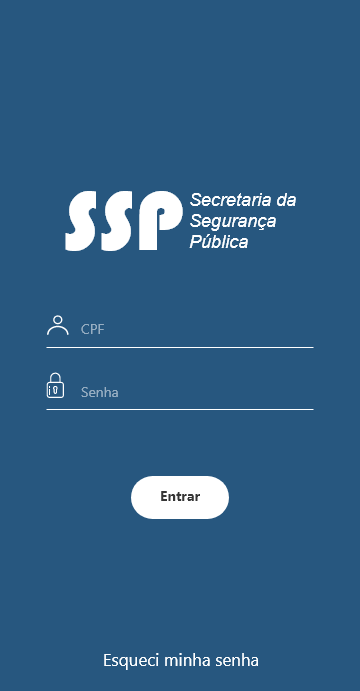
\includegraphics[width=.9\linewidth]{imagens/prototipoLogin}
            \label{fig: Tela de login}
        \end{minipage}
        \begin{minipage}{.3\textwidth}
            \centering
            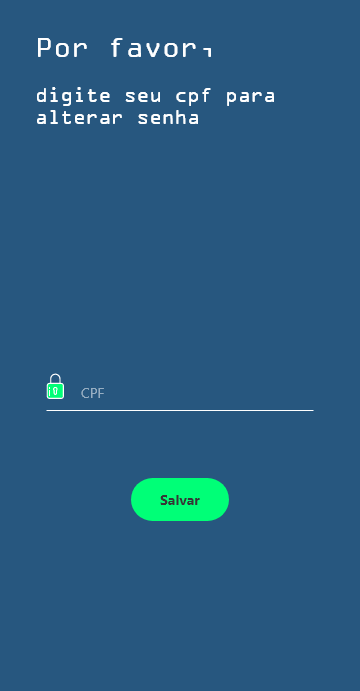
\includegraphics[width=.9\linewidth]{imagens/prototipoEsqueciSenha}
            \label{fig: Tela esqueci minha senha}
        \end{minipage}%
        \begin{minipage}{.3\textwidth}
            \centering
            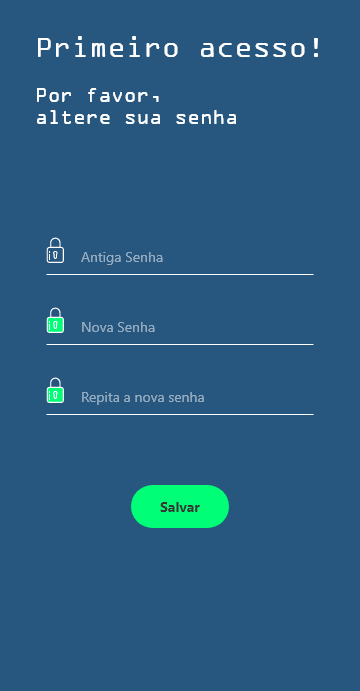
\includegraphics[width=.9\linewidth]{imagens/prototipoPrimeiroAcesso}
            \label{fig: Tela de primeira autenticação}
        \end{minipage}
        \caption{Prototipação 001}
    \end{figure}

    \begin{figure}[H]
        \centering
        \begin{minipage}{.3\textwidth}
            \centering
            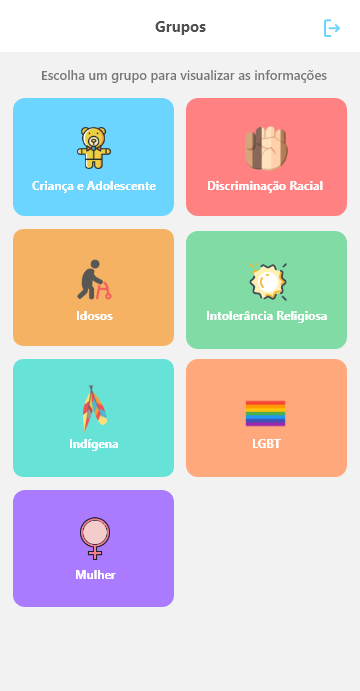
\includegraphics[width=.9\linewidth]{imagens/prototipoInicio}
            \label{fig: Tela inicial}
        \end{minipage}
        \begin{minipage}{.3\textwidth}
            \centering
            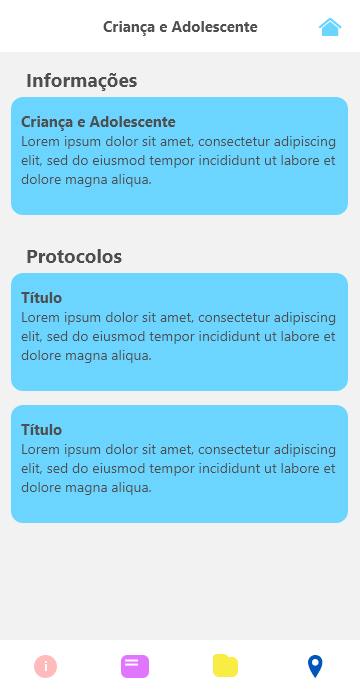
\includegraphics[width=.9\linewidth]{imagens/prototipoProtocolos}
            \label{fig: Tela de protocolos}
        \end{minipage}%
        \begin{minipage}{.3\textwidth}
            \centering
            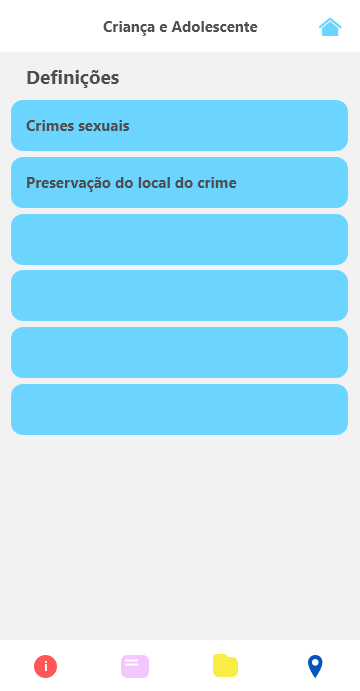
\includegraphics[width=.9\linewidth]{imagens/prototipoDefinicoes}
            \label{fig: Tela de definições}
        \end{minipage}
        \caption{Prototipação 002}
    \end{figure}

    \begin{figure}[H]
        \centering
        \begin{minipage}{.3\textwidth}
            \centering
            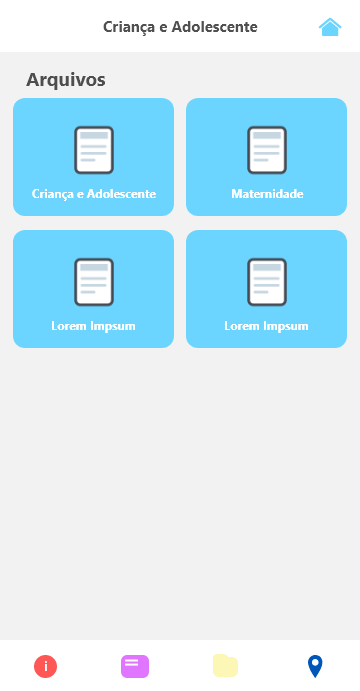
\includegraphics[width=.9\linewidth]{imagens/prototipoArquivos}
            \label{fig: Tela de arquivos}
        \end{minipage}
        \begin{minipage}{.3\textwidth}
            \centering
            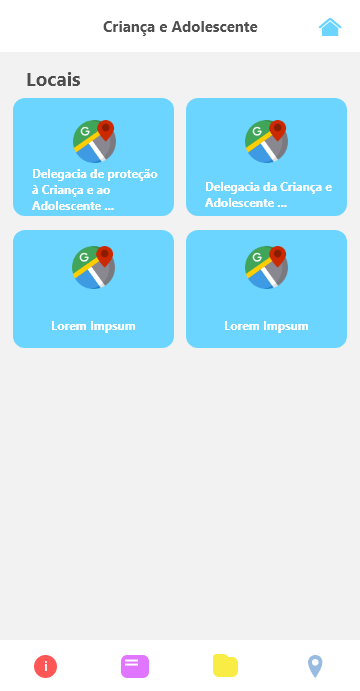
\includegraphics[width=.9\linewidth]{imagens/prototipLocais}
            \label{fig: Tela locais}
        \end{minipage}%
        \begin{minipage}{.3\textwidth}
            \centering
            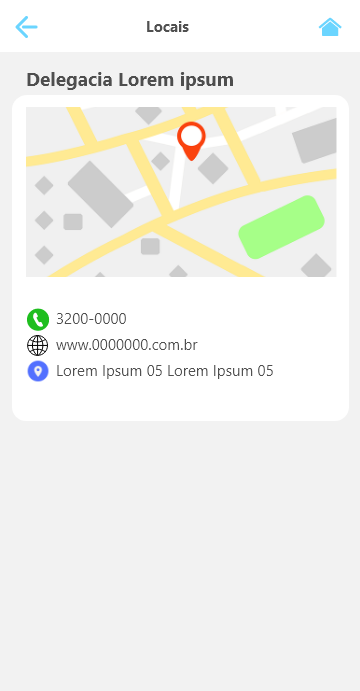
\includegraphics[width=.9\linewidth]{imagens/prototipoLocal}
            \label{fig: Tela de detalhamento local}
        \end{minipage}
        \caption{Prototipação 003}
    \end{figure}
% ----------------------------------------------------------
% Glossário
% ----------------------------------------------------------
%
% Consulte o manual da classe abntex2 para orientações sobre o glossário.
%
%\glossary

%---------------------------------------------------------------------
% INDICE REMISSIVO
%---------------------------------------------------------------------
    \phantompart
    \printindex
%---------------------------------------------------------------------

\end{document}
\grid
